\documentclass[11pt]{article}
\usepackage{amsmath,amssymb,xspace,epsfig}
\usepackage{algorithm}
\usepackage{algpseudocode}
\usepackage{algorithmicx}
\usepackage{graphicx}
\usepackage{subfigure}
\usepackage{natbib}
\usepackage[colorlinks]{hyperref}
\usepackage{makecell}
\usepackage[colorinlistoftodos]{todonotes}

\graphicspath{{plots/}}

\hypersetup{
     colorlinks = true,
     linkcolor = blue,
     anchorcolor = blue,
     citecolor = blue,
     filecolor = blue,
     urlcolor = blue
}

\textwidth 6.5in \textheight 9.05in \oddsidemargin 0.0in
\evensidemargin 0.0in \topmargin -0.55in
\addtolength{\textwidth}{2.5mm} \addtolength{\columnsep}{2mm}

\title{Report of Assignment 2}
\author{Haoyang Zhang (hz333), Qi Wu (qw142), Shengjie Li (sl1560)}

\begin{document}
\date{\today}
\maketitle

\subsection*{Problem1: XOR}
\begin{enumerate}
	\item 
	\texttt{1} : input neuron will fire with a delay of 6ms. \\
	\texttt{0} : input neuron will fire with a delay of 0ms.
	\item
	\texttt{1} : input neuron will fire with a higher rate, like \texttt{200 Hz}.\\
	\texttt{0} : input neuron will fire with a lower rate, like \texttt{100 Hz}.
	\item
	The 3-layer SNN (code available in \texttt{./code/xorBCM.py} and \texttt{./code/stdp.py}) we build including 2 Poisson neurons at input layer, several LIF neurons at hidden layer and 1 LIF neuron at output layer. The exact network topology is introduced in our answers to the next two questions.
	\item
	In Hebbian learning part (code available in \texttt{./code/xorBCM.py}), the coding method of input and output is rate coding. More specifically, we encode input \texttt{1} with \texttt{200 Hz}, and \texttt{0} with \texttt{100 Hz}. For the output decoding, we use \texttt{150 Hz} to represent \texttt{1}, and \texttt{40 Hz} to represent \texttt{0}. The threshold between \texttt{1} and \texttt{0} is set as \texttt{95 Hz}. The network topology is $(2, 2, 1)$. (See Fig. \ref{fig.xorBCMtopo}.) We use BCM rule to train the network. To train the network, we add 3 teaching input currents totally, 2 for the hidden layer and 1 for output layer. The teaching input currents directly inject into the "student" neuron to force it firing or not. We constrain the hidden neuron to represent $h_1 = \lnot x \land y, h_2 = x \land \lnot y$, and therefore the output neuron acts as $z = h_1 \lor h_2$. (See Table. \ref{table.xorBCMtruth}) For ease of training, we further trained this network layer by layer, and constrained the weights being symmetric in terms of $x$ and $y$.
	\begin{figure}[htbp]
	\centering
        \tikzset{every picture/.style={line width=0.75pt}} %set default line width to 0.75pt        

        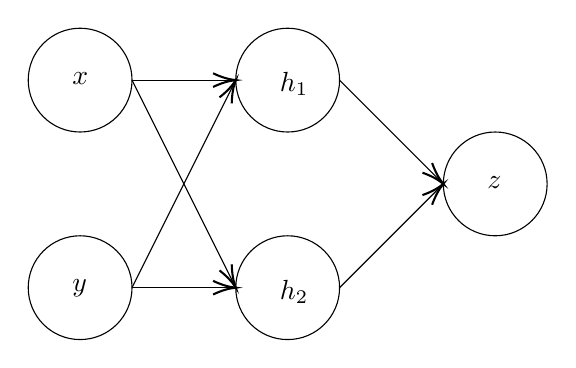
\begin{tikzpicture}[x=0.75pt,y=0.75pt,yscale=-1,xscale=1]
        %uncomment if require: \path (0,300); %set diagram left start at 0, and has height of 300

        %Shape: Circle [id:dp8890499279534472] 
        \draw   (50,75) .. controls (50,61.19) and (61.19,50) .. (75,50) .. controls (88.81,50) and (100,61.19) .. (100,75) .. controls (100,88.81) and (88.81,100) .. (75,100) .. controls (61.19,100) and (50,88.81) .. (50,75) -- cycle ;
        %Shape: Circle [id:dp9166815346577286] 
        \draw   (50,175) .. controls (50,161.19) and (61.19,150) .. (75,150) .. controls (88.81,150) and (100,161.19) .. (100,175) .. controls (100,188.81) and (88.81,200) .. (75,200) .. controls (61.19,200) and (50,188.81) .. (50,175) -- cycle ;
        %Shape: Circle [id:dp6119856338926952] 
        \draw   (150,75) .. controls (150,61.19) and (161.19,50) .. (175,50) .. controls (188.81,50) and (200,61.19) .. (200,75) .. controls (200,88.81) and (188.81,100) .. (175,100) .. controls (161.19,100) and (150,88.81) .. (150,75) -- cycle ;
        %Shape: Circle [id:dp7239420187339329] 
        \draw   (150,175) .. controls (150,161.19) and (161.19,150) .. (175,150) .. controls (188.81,150) and (200,161.19) .. (200,175) .. controls (200,188.81) and (188.81,200) .. (175,200) .. controls (161.19,200) and (150,188.81) .. (150,175) -- cycle ;
        %Shape: Circle [id:dp9694660742855763] 
        \draw   (250,125) .. controls (250,111.19) and (261.19,100) .. (275,100) .. controls (288.81,100) and (300,111.19) .. (300,125) .. controls (300,138.81) and (288.81,150) .. (275,150) .. controls (261.19,150) and (250,138.81) .. (250,125) -- cycle ;
        %Straight Lines [id:da16263740176524122] 
        \draw    (100,75) -- (148,75) ;
        \draw [shift={(150,75)}, rotate = 180] [color={rgb, 255:red, 0; green, 0; blue, 0 }  ][line width=0.75]    (10.93,-3.29) .. controls (6.95,-1.4) and (3.31,-0.3) .. (0,0) .. controls (3.31,0.3) and (6.95,1.4) .. (10.93,3.29)   ;
        %Straight Lines [id:da7077843419925032] 
        \draw    (100,175) -- (149.11,76.79) ;
        \draw [shift={(150,75)}, rotate = 476.57] [color={rgb, 255:red, 0; green, 0; blue, 0 }  ][line width=0.75]    (10.93,-3.29) .. controls (6.95,-1.4) and (3.31,-0.3) .. (0,0) .. controls (3.31,0.3) and (6.95,1.4) .. (10.93,3.29)   ;
        %Straight Lines [id:da04055662031604834] 
        \draw    (100,75) -- (149.11,173.21) ;
        \draw [shift={(150,175)}, rotate = 243.43] [color={rgb, 255:red, 0; green, 0; blue, 0 }  ][line width=0.75]    (10.93,-3.29) .. controls (6.95,-1.4) and (3.31,-0.3) .. (0,0) .. controls (3.31,0.3) and (6.95,1.4) .. (10.93,3.29)   ;
        %Straight Lines [id:da9834041914738147] 
        \draw    (100,175) -- (148,175) ;
        \draw [shift={(150,175)}, rotate = 180] [color={rgb, 255:red, 0; green, 0; blue, 0 }  ][line width=0.75]    (10.93,-3.29) .. controls (6.95,-1.4) and (3.31,-0.3) .. (0,0) .. controls (3.31,0.3) and (6.95,1.4) .. (10.93,3.29)   ;
        %Straight Lines [id:da8071598107998539] 
        \draw    (200,75) -- (248.59,123.59) ;
        \draw [shift={(250,125)}, rotate = 225] [color={rgb, 255:red, 0; green, 0; blue, 0 }  ][line width=0.75]    (10.93,-3.29) .. controls (6.95,-1.4) and (3.31,-0.3) .. (0,0) .. controls (3.31,0.3) and (6.95,1.4) .. (10.93,3.29)   ;
        %Straight Lines [id:da1547600119304655] 
        \draw    (200,175) -- (248.59,126.41) ;
        \draw [shift={(250,125)}, rotate = 495] [color={rgb, 255:red, 0; green, 0; blue, 0 }  ][line width=0.75]    (10.93,-3.29) .. controls (6.95,-1.4) and (3.31,-0.3) .. (0,0) .. controls (3.31,0.3) and (6.95,1.4) .. (10.93,3.29)   ;

        % Text Node
        \draw (270,120) node [anchor=north west][inner sep=0.75pt]   [align=left] {$\displaystyle z$};
        % Text Node
        \draw (170,170) node [anchor=north west][inner sep=0.75pt]   [align=left] {$\displaystyle h_{2}$};
        % Text Node
        \draw (170,70) node [anchor=north west][inner sep=0.75pt]   [align=left] {$\displaystyle h_{1}$};
        % Text Node
        \draw (70,170) node [anchor=north west][inner sep=0.75pt]   [align=left] {$\displaystyle y$};
        % Text Node
        \draw (70,70) node [anchor=north west][inner sep=0.75pt]   [align=left] {$\displaystyle x$};

        \end{tikzpicture}

        \caption{the topology of xorBCM network}
        \label{fig.xorBCMtopo}
	\end{figure}
    \begin{table}[htbp]
        \centering
        \begin{tabular}{ll|ll|l}
        $x$ & $y$ & $h_1$ & $h_2$ & $z$ \\ \hline
        0 & 0 & 0  & 0  & 0 \\
        0 & 1 & 1  & 0  & 1 \\
        1 & 0 & 0  & 1  & 1 \\
        1 & 1 & 0  & 0  & 0
        \end{tabular}
        \caption{the truth table of xorBCM network}
        \label{table.xorBCMtruth}
    \end{table}

	The result is shown in Fig. \ref{fig.xorBCMspiking} and \ref{fig.xorBCMrate}. The output neuron fires at averaged about \texttt{50 Hz} with input \texttt{(0, 0)}, \texttt{160 Hz} with \texttt{(0, 1)}, \texttt{150 Hz} with \texttt{(1, 0)}, and \texttt{40 Hz} with \texttt{(1, 1)}. Namely, the output neuron performs the $\oplus$ operation of the inputs.
	
	\begin{figure}[htbp]
		\centering
		\subfigure[input \texttt{(0, 0)}]{
		\label{fig.xorBCMspiking00}
		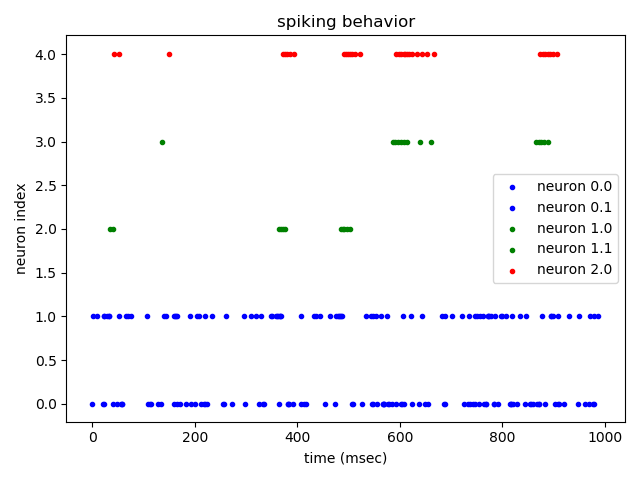
\includegraphics[width=.48\textwidth]{xorBCM.input3.iter0.spikeList.png}}
		\subfigure[input \texttt{(0, 1)}]{
		\label{fig.xorBCMspiking01}
		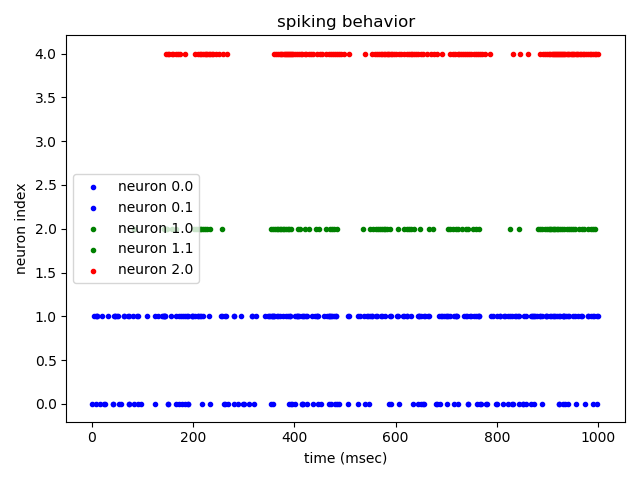
\includegraphics[width=.48\textwidth]{xorBCM.input2.iter0.spikeList.png}}
		\subfigure[input \texttt{(1, 0)}]{
		\label{fig.xorBCMspiking10}
		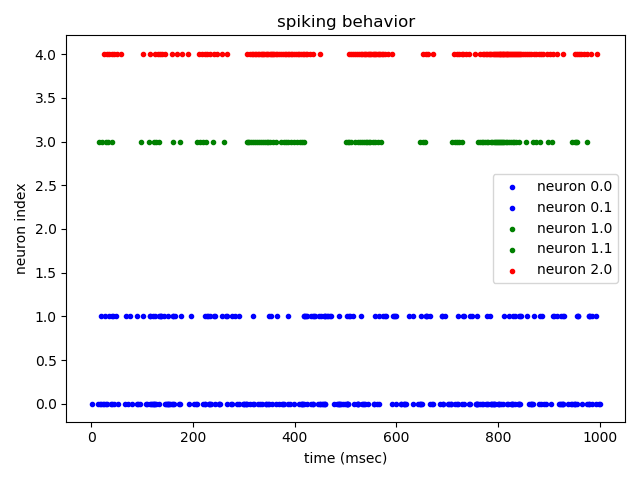
\includegraphics[width=.48\textwidth]{xorBCM.input1.iter0.spikeList.png}}
		\subfigure[input \texttt{(1, 1)}]{
		\label{fig.xorBCMspiking11}
		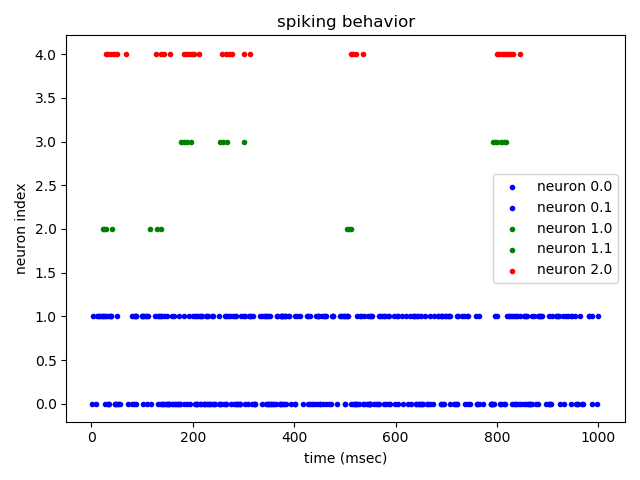
\includegraphics[width=.48\textwidth]{xorBCM.input0.iter0.spikeList.png}}
		\caption{spiking behavior of xorBCM network}
		\label{fig.xorBCMspiking}
	\end{figure}
	
	\begin{figure}[H]
	\centering
	    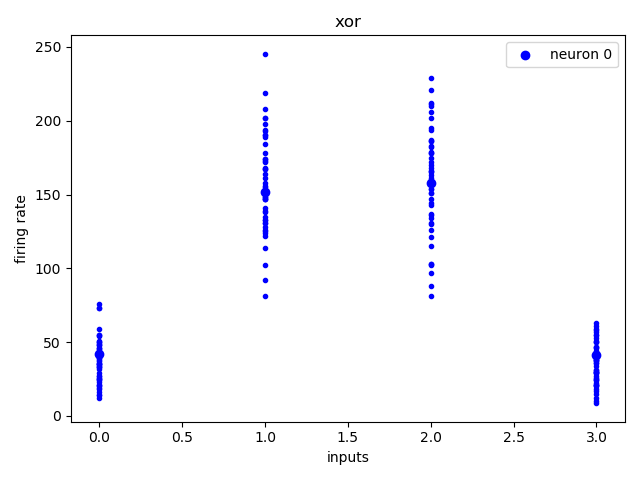
\includegraphics[width=.48\textwidth]{xorBCM.iter49.rate.png}
	    \caption{averaged spiking rate of xor neuron (trained by BCM) of 50 iterations, where inputs 0.0, 1.0, 2.0, and 3.0 represent input \texttt{(1, 1)}, \texttt{(1, 0)}, \texttt{(0, 1)}, and \texttt{(0, 0)}, respectively}
	    \label{fig.xorBCMrate}
	\end{figure}

	\item
	In STDP learning part (code available in \texttt{./code/stdp.py}), we also use rate coding to code the input and output. For the input neuron, we encode \texttt{1} with \texttt{125 Hz}, and \texttt{0} with \texttt{25 Hz}. For output neuron,  \texttt{1} fall in range \texttt{100-150Hz}, and \texttt{0} fall in \texttt{0-30HZ}. The network topology is $(2, 10, 1)$. Also, we add a teaching input as supervised data to train the network. For teaching input, we use \texttt{250 Hz} to represent \texttt{1} and \texttt{50 Hz} to represent \texttt{0}. In training, we first run the network with 1000 ms and get the spike train of each neuron. Next, we update the weight of synapse between the input layer and the hidden layer with unsupervised STDP \cite[]{Morrison2008}. Then, we use the teaching input to update the synapse between the hidden layer and the output layer with supervised STDP, ReSuMe \cite[]{10.1162/neco.2009.11-08-901}. The update rule is as follows: 
	$$\Delta w(t) = [S_d(t) - S_o(t)][a_d + \int_0^\infty a^{post}S_h(t-s)\text{d}s]$$
	Where $S_d$, $S_o$, and $S_h$ are the spike train of the teaching input, the output neuron and the hidden neuron. We set $a_d = 0$ and $a^{post} = 0.005$.
	
	The result is shown in Fig. \ref{fig.stdpSpiking}.
	\begin{figure}[H]
		\centering
		\subfigure[input \texttt{(0, 0)}]{
		\label{fig.stdpSpiking00}
		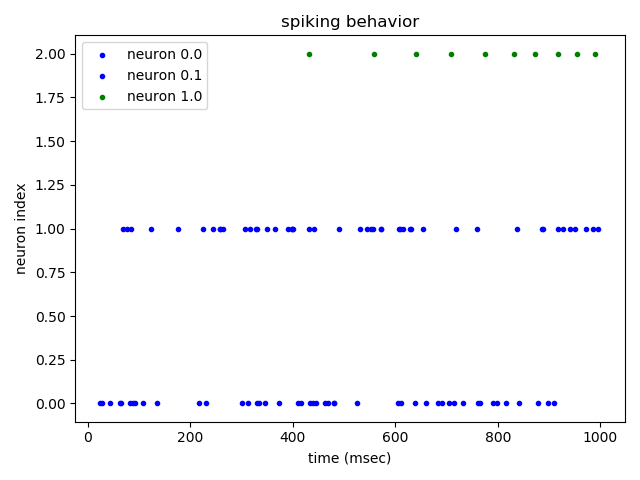
\includegraphics[width=.48\textwidth]{stdp.input3.iter5.spikeList.png}}
		\subfigure[input \texttt{(0, 1)}]{
		\label{fig.stdpSpiking01}
		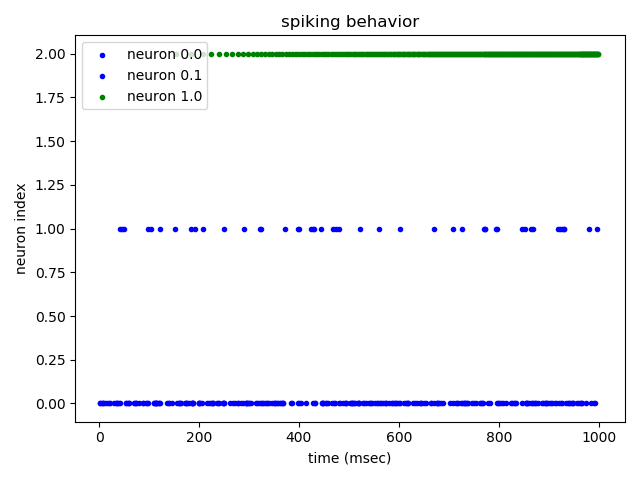
\includegraphics[width=.48\textwidth]{stdp.input1.iter5.spikeList.png}}
		\subfigure[input \texttt{(1, 0)}]{
		\label{fig.stdpSpiking10}
		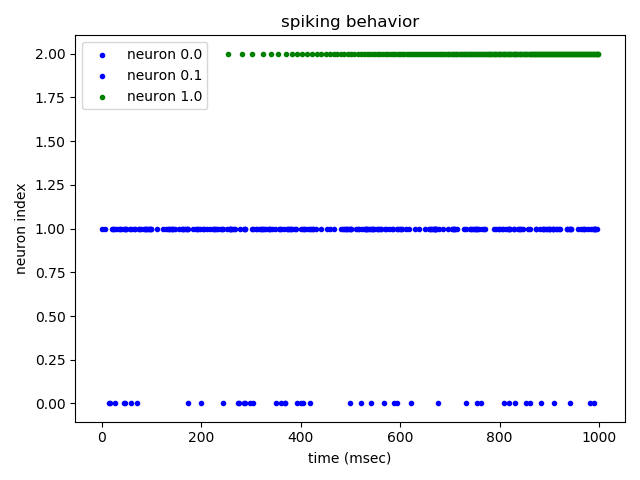
\includegraphics[width=.48\textwidth]{stdp.input2.iter4.spikeList.png}}
		\subfigure[input \texttt{(1, 1)}]{
		\label{fig.stdpSpiking11}
		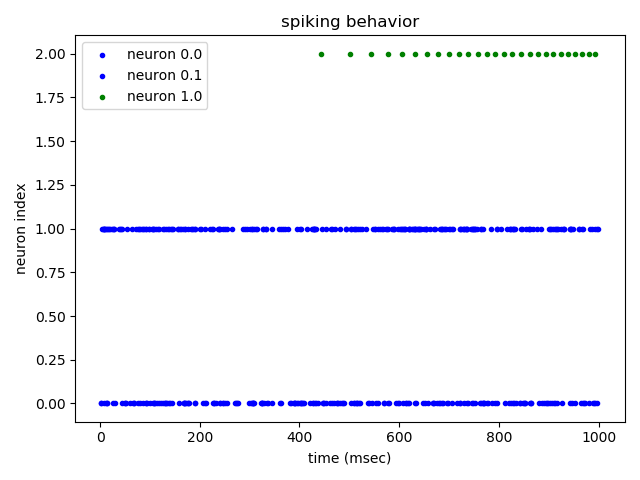
\includegraphics[width=.48\textwidth]{stdp.input0.iter1.spikeList.png}}
		\caption{spiking behavior of STDP network (neurons 0.0 and 0.1 are Poisson input neurons and neoron 1.0 is the output neuron)}
		\label{fig.stdpSpiking}
	\end{figure}

\end{enumerate}

\subsection*{Problem2: Line detector}
    We construct the ``on-off'' cell with two parts: the convolutional part and the Poisson part. The convolutional part takes a portion of the whole inputs and convolutes it with a kernel (See Table. \ref{table.onoffKernel}.) to perform the receptive field of the ``on-off'' cell. Then, Poisson part takes the output of the convolutional part as inputs, and emits spikes with the rate proportional to inputs (in range \texttt{10 Hz} - \texttt{200 Hz}). (See Fig. \ref{fig.onoffStructure}.)  To decode the outputs, we still use the rate coding scheme. Specifically, we set the threshold as \texttt{150 Hz}.
    
    \begin{table}[htbp]
    \centering
        \begin{tabular}{|l|l|l|}
        \hline
        -1 & -2 & -1 \\ \hline
        -2 & 12 & -2 \\ \hline
        -1 & -2 & -1 \\ \hline
        \end{tabular}
        \caption{convolutional kernel of ``on-off'' cells}
        \label{table.onoffKernel}
    \end{table}
    \begin{figure}[htbp]
    \centering
        \tikzset{every picture/.style={line width=0.75pt}} %set default line width to 0.75pt        
    
        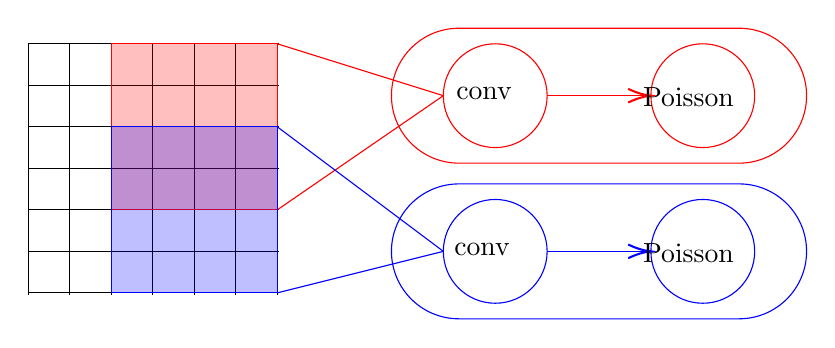
\begin{tikzpicture}[x=0.75pt,y=0.75pt,yscale=-1,xscale=1]
        %uncomment if require: \path (0,300); %set diagram left start at 0, and has height of 300
    
        %Shape: Grid [id:dp08257542002902629] 
        \draw  [draw opacity=0] (50,50) -- (171,50) -- (171,171) -- (50,171) -- cycle ; \draw   (50,50) -- (50,171)(70,50) -- (70,171)(90,50) -- (90,171)(110,50) -- (110,171)(130,50) -- (130,171)(150,50) -- (150,171)(170,50) -- (170,171) ; \draw   (50,50) -- (171,50)(50,70) -- (171,70)(50,90) -- (171,90)(50,110) -- (171,110)(50,130) -- (171,130)(50,150) -- (171,150)(50,170) -- (171,170) ; \draw    ;
        %Shape: Rectangle [id:dp2550056626515027] 
        \draw  [color={rgb, 255:red, 255; green, 0; blue, 0 }  ,draw opacity=1 ][fill={rgb, 255:red, 255; green, 0; blue, 0 }  ,fill opacity=0.25 ] (90,50) -- (170,50) -- (170,130) -- (90,130) -- cycle ;
        %Shape: Circle [id:dp15272694241606977] 
        \draw  [color={rgb, 255:red, 255; green, 0; blue, 0 }  ,draw opacity=1 ] (250,75) .. controls (250,61.19) and (261.19,50) .. (275,50) .. controls (288.81,50) and (300,61.19) .. (300,75) .. controls (300,88.81) and (288.81,100) .. (275,100) .. controls (261.19,100) and (250,88.81) .. (250,75) -- cycle ;
        %Shape: Circle [id:dp9234562563770208] 
        \draw  [color={rgb, 255:red, 255; green, 0; blue, 0 }  ,draw opacity=1 ] (350,75) .. controls (350,61.19) and (361.19,50) .. (375,50) .. controls (388.81,50) and (400,61.19) .. (400,75) .. controls (400,88.81) and (388.81,100) .. (375,100) .. controls (361.19,100) and (350,88.81) .. (350,75) -- cycle ;
        %Straight Lines [id:da885046024771726] 
        \draw [color={rgb, 255:red, 255; green, 0; blue, 0 }  ,draw opacity=1 ]   (170,50) -- (250,75) ;
        %Straight Lines [id:da27540496385556823] 
        \draw [color={rgb, 255:red, 255; green, 0; blue, 0 }  ,draw opacity=1 ]   (170,130) -- (250,75) ;
        %Shape: Rectangle [id:dp9011595559434677] 
        \draw  [color={rgb, 255:red, 0; green, 0; blue, 255 }  ,draw opacity=1 ][fill={rgb, 255:red, 0; green, 0; blue, 255 }  ,fill opacity=0.25 ] (90,90) -- (170,90) -- (170,170) -- (90,170) -- cycle ;
        %Shape: Circle [id:dp23323185533775614] 
        \draw  [color={rgb, 255:red, 0; green, 0; blue, 255 }  ,draw opacity=1 ] (250,150) .. controls (250,136.19) and (261.19,125) .. (275,125) .. controls (288.81,125) and (300,136.19) .. (300,150) .. controls (300,163.81) and (288.81,175) .. (275,175) .. controls (261.19,175) and (250,163.81) .. (250,150) -- cycle ;
        %Straight Lines [id:da35174209207771545] 
        \draw [color={rgb, 255:red, 0; green, 0; blue, 255 }  ,draw opacity=1 ]   (170,90) -- (250,150) ;
        %Straight Lines [id:da7971372221069235] 
        \draw [color={rgb, 255:red, 0; green, 0; blue, 255 }  ,draw opacity=1 ]   (170,170) -- (250,150) ;
        %Straight Lines [id:da4735686700467645] 
        \draw [color={rgb, 255:red, 255; green, 0; blue, 0 }  ,draw opacity=1 ]   (300,75) -- (348,75) ;
        \draw [shift={(350,75)}, rotate = 180] [color={rgb, 255:red, 255; green, 0; blue, 0 }  ,draw opacity=1 ][line width=0.75]    (10.93,-3.29) .. controls (6.95,-1.4) and (3.31,-0.3) .. (0,0) .. controls (3.31,0.3) and (6.95,1.4) .. (10.93,3.29)   ;
        %Shape: Circle [id:dp25455676950536965] 
        \draw  [color={rgb, 255:red, 0; green, 0; blue, 255 }  ,draw opacity=1 ] (350,150) .. controls (350,136.19) and (361.19,125) .. (375,125) .. controls (388.81,125) and (400,136.19) .. (400,150) .. controls (400,163.81) and (388.81,175) .. (375,175) .. controls (361.19,175) and (350,163.81) .. (350,150) -- cycle ;
        %Straight Lines [id:da3048723294003448] 
        \draw [color={rgb, 255:red, 0; green, 0; blue, 255 }  ,draw opacity=1 ]   (300,150) -- (348,150) ;
        \draw [shift={(350,150)}, rotate = 180] [color={rgb, 255:red, 0; green, 0; blue, 255 }  ,draw opacity=1 ][line width=0.75]    (10.93,-3.29) .. controls (6.95,-1.4) and (3.31,-0.3) .. (0,0) .. controls (3.31,0.3) and (6.95,1.4) .. (10.93,3.29)   ;
        %Rounded Rect [id:dp5517604958269509] 
        \draw  [color={rgb, 255:red, 255; green, 0; blue, 0 }  ,draw opacity=1 ] (225,75) .. controls (225,57.05) and (239.55,42.5) .. (257.5,42.5) -- (392.5,42.5) .. controls (410.45,42.5) and (425,57.05) .. (425,75) -- (425,75) .. controls (425,92.95) and (410.45,107.5) .. (392.5,107.5) -- (257.5,107.5) .. controls (239.55,107.5) and (225,92.95) .. (225,75) -- cycle ;
        %Rounded Rect [id:dp2087356998306653] 
        \draw  [color={rgb, 255:red, 0; green, 0; blue, 255 }  ,draw opacity=1 ] (225,150) .. controls (225,132.05) and (239.55,117.5) .. (257.5,117.5) -- (392.5,117.5) .. controls (410.45,117.5) and (425,132.05) .. (425,150) -- (425,150) .. controls (425,167.95) and (410.45,182.5) .. (392.5,182.5) -- (257.5,182.5) .. controls (239.55,182.5) and (225,167.95) .. (225,150) -- cycle ;
    
    
        % Text Node
        \draw (345,145) node [anchor=north west][inner sep=0.75pt]   [align=left] {Poisson};
        % Text Node
        \draw (254,145) node [anchor=north west][inner sep=0.75pt]   [align=left] {conv};
        % Text Node
        \draw (345,70) node [anchor=north west][inner sep=0.75pt]   [align=left] {Poisson};
        % Text Node
        \draw (255,70) node [anchor=north west][inner sep=0.75pt]   [align=left] {conv};
        
        \end{tikzpicture}
        \caption{two ``on-off'' cells}
        \label{fig.onoffStructure}
    \end{figure}
    
    For ease of denotation, call the ``on-off'' cells that are excited if on-center, off-surround On Cell, and the other type Off Cell.
    
    We consider building an line detector to detect an horizontal line. Namely, the detector neuron will be excited if a row of On Cells are excited, which indicates existing at least a line, and the two rows of Off Cells, next to the given row, are also excited, which indicates existing no more than a line. Therefore, the topology of this network is sparse. (See Fig. \ref{fig.lineTopo}.) More specifically, we set the weight of On Cells to detector cells as $1$, and Off Cells to detector cells as $0.5$.
    \begin{figure}[htbp]
    \centering
        
        \tikzset{every picture/.style={line width=0.75pt}} %set default line width to 0.75pt        
    
        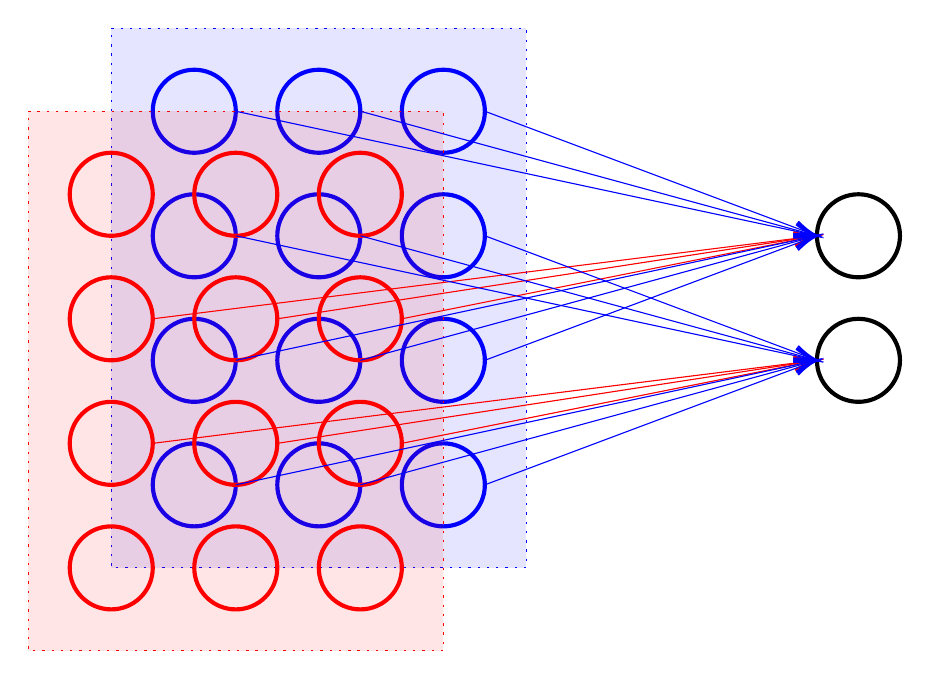
\begin{tikzpicture}[x=0.75pt,y=0.75pt,yscale=-1,xscale=1]
        %uncomment if require: \path (0,427); %set diagram left start at 0, and has height of 427
    
        %Shape: Rectangle [id:dp8776322035012474] 
        \draw  [color={rgb, 255:red, 0; green, 0; blue, 255 }  ,draw opacity=1 ][fill={rgb, 255:red, 0; green, 0; blue, 255 }  ,fill opacity=0.1 ][dash pattern={on 0.84pt off 2.51pt}] (65,25) -- (265,25) -- (265,285) -- (65,285) -- cycle ;
        %Shape: Circle [id:dp3441119285512326] 
        \draw  [color={rgb, 255:red, 0; green, 0; blue, 255 }  ,draw opacity=1 ][line width=1.5]  (85,65) .. controls (85,53.95) and (93.95,45) .. (105,45) .. controls (116.05,45) and (125,53.95) .. (125,65) .. controls (125,76.05) and (116.05,85) .. (105,85) .. controls (93.95,85) and (85,76.05) .. (85,65) -- cycle ;
        %Shape: Circle [id:dp9560561330771498] 
        \draw  [color={rgb, 255:red, 0; green, 0; blue, 255 }  ,draw opacity=1 ][line width=1.5]  (145,65) .. controls (145,53.95) and (153.95,45) .. (165,45) .. controls (176.05,45) and (185,53.95) .. (185,65) .. controls (185,76.05) and (176.05,85) .. (165,85) .. controls (153.95,85) and (145,76.05) .. (145,65) -- cycle ;
        %Shape: Circle [id:dp9782910750486635] 
        \draw  [color={rgb, 255:red, 0; green, 0; blue, 255 }  ,draw opacity=1 ][line width=1.5]  (205,65) .. controls (205,53.95) and (213.95,45) .. (225,45) .. controls (236.05,45) and (245,53.95) .. (245,65) .. controls (245,76.05) and (236.05,85) .. (225,85) .. controls (213.95,85) and (205,76.05) .. (205,65) -- cycle ;
        %Shape: Circle [id:dp8165829031400178] 
        \draw  [color={rgb, 255:red, 0; green, 0; blue, 255 }  ,draw opacity=1 ][line width=1.5]  (85,125) .. controls (85,113.95) and (93.95,105) .. (105,105) .. controls (116.05,105) and (125,113.95) .. (125,125) .. controls (125,136.05) and (116.05,145) .. (105,145) .. controls (93.95,145) and (85,136.05) .. (85,125) -- cycle ;
        %Shape: Circle [id:dp4171352692422807] 
        \draw  [color={rgb, 255:red, 0; green, 0; blue, 255 }  ,draw opacity=1 ][line width=1.5]  (145,125) .. controls (145,113.95) and (153.95,105) .. (165,105) .. controls (176.05,105) and (185,113.95) .. (185,125) .. controls (185,136.05) and (176.05,145) .. (165,145) .. controls (153.95,145) and (145,136.05) .. (145,125) -- cycle ;
        %Shape: Circle [id:dp22097927486305302] 
        \draw  [color={rgb, 255:red, 0; green, 0; blue, 255 }  ,draw opacity=1 ][line width=1.5]  (205,125) .. controls (205,113.95) and (213.95,105) .. (225,105) .. controls (236.05,105) and (245,113.95) .. (245,125) .. controls (245,136.05) and (236.05,145) .. (225,145) .. controls (213.95,145) and (205,136.05) .. (205,125) -- cycle ;
        %Shape: Circle [id:dp7065222144700798] 
        \draw  [color={rgb, 255:red, 0; green, 0; blue, 255 }  ,draw opacity=1 ][line width=1.5]  (85,185) .. controls (85,173.95) and (93.95,165) .. (105,165) .. controls (116.05,165) and (125,173.95) .. (125,185) .. controls (125,196.05) and (116.05,205) .. (105,205) .. controls (93.95,205) and (85,196.05) .. (85,185) -- cycle ;
        %Shape: Circle [id:dp5998246771102977] 
        \draw  [color={rgb, 255:red, 0; green, 0; blue, 255 }  ,draw opacity=1 ][line width=1.5]  (145,185) .. controls (145,173.95) and (153.95,165) .. (165,165) .. controls (176.05,165) and (185,173.95) .. (185,185) .. controls (185,196.05) and (176.05,205) .. (165,205) .. controls (153.95,205) and (145,196.05) .. (145,185) -- cycle ;
        %Shape: Circle [id:dp5489065208631285] 
        \draw  [color={rgb, 255:red, 0; green, 0; blue, 255 }  ,draw opacity=1 ][line width=1.5]  (205,185) .. controls (205,173.95) and (213.95,165) .. (225,165) .. controls (236.05,165) and (245,173.95) .. (245,185) .. controls (245,196.05) and (236.05,205) .. (225,205) .. controls (213.95,205) and (205,196.05) .. (205,185) -- cycle ;
        %Shape: Circle [id:dp4567571142201603] 
        \draw  [color={rgb, 255:red, 0; green, 0; blue, 255 }  ,draw opacity=1 ][line width=1.5]  (85,245) .. controls (85,233.95) and (93.95,225) .. (105,225) .. controls (116.05,225) and (125,233.95) .. (125,245) .. controls (125,256.05) and (116.05,265) .. (105,265) .. controls (93.95,265) and (85,256.05) .. (85,245) -- cycle ;
        %Shape: Circle [id:dp17649529374759254] 
        \draw  [color={rgb, 255:red, 0; green, 0; blue, 255 }  ,draw opacity=1 ][line width=1.5]  (145,245) .. controls (145,233.95) and (153.95,225) .. (165,225) .. controls (176.05,225) and (185,233.95) .. (185,245) .. controls (185,256.05) and (176.05,265) .. (165,265) .. controls (153.95,265) and (145,256.05) .. (145,245) -- cycle ;
        %Shape: Circle [id:dp9155649783253414] 
        \draw  [color={rgb, 255:red, 0; green, 0; blue, 255 }  ,draw opacity=1 ][line width=1.5]  (205,245) .. controls (205,233.95) and (213.95,225) .. (225,225) .. controls (236.05,225) and (245,233.95) .. (245,245) .. controls (245,256.05) and (236.05,265) .. (225,265) .. controls (213.95,265) and (205,256.05) .. (205,245) -- cycle ;
    
        %Shape: Rectangle [id:dp45168134887741673] 
        \draw  [color={rgb, 255:red, 255; green, 0; blue, 0 }  ,draw opacity=1 ][fill={rgb, 255:red, 255; green, 0; blue, 0 }  ,fill opacity=0.1 ][dash pattern={on 0.84pt off 2.51pt}] (25,65) -- (225,65) -- (225,325) -- (25,325) -- cycle ;
        %Shape: Circle [id:dp7164817511162116] 
        \draw  [color={rgb, 255:red, 255; green, 0; blue, 0 }  ,draw opacity=1 ][fill={rgb, 255:red, 255; green, 0; blue, 0 }  ,fill opacity=0 ][line width=1.5]  (45,105) .. controls (45,93.95) and (53.95,85) .. (65,85) .. controls (76.05,85) and (85,93.95) .. (85,105) .. controls (85,116.05) and (76.05,125) .. (65,125) .. controls (53.95,125) and (45,116.05) .. (45,105) -- cycle ;
        %Shape: Circle [id:dp0666800049224312] 
        \draw  [color={rgb, 255:red, 255; green, 0; blue, 0 }  ,draw opacity=1 ][fill={rgb, 255:red, 255; green, 0; blue, 0 }  ,fill opacity=0 ][line width=1.5]  (105,105) .. controls (105,93.95) and (113.95,85) .. (125,85) .. controls (136.05,85) and (145,93.95) .. (145,105) .. controls (145,116.05) and (136.05,125) .. (125,125) .. controls (113.95,125) and (105,116.05) .. (105,105) -- cycle ;
        %Shape: Circle [id:dp27202414155480326] 
        \draw  [color={rgb, 255:red, 255; green, 0; blue, 0 }  ,draw opacity=1 ][fill={rgb, 255:red, 255; green, 0; blue, 0 }  ,fill opacity=0 ][line width=1.5]  (165,105) .. controls (165,93.95) and (173.95,85) .. (185,85) .. controls (196.05,85) and (205,93.95) .. (205,105) .. controls (205,116.05) and (196.05,125) .. (185,125) .. controls (173.95,125) and (165,116.05) .. (165,105) -- cycle ;
        %Shape: Circle [id:dp5715628596434843] 
        \draw  [color={rgb, 255:red, 255; green, 0; blue, 0 }  ,draw opacity=1 ][fill={rgb, 255:red, 255; green, 0; blue, 0 }  ,fill opacity=0 ][line width=1.5]  (45,165) .. controls (45,153.95) and (53.95,145) .. (65,145) .. controls (76.05,145) and (85,153.95) .. (85,165) .. controls (85,176.05) and (76.05,185) .. (65,185) .. controls (53.95,185) and (45,176.05) .. (45,165) -- cycle ;
        %Shape: Circle [id:dp025322892487183335] 
        \draw  [color={rgb, 255:red, 255; green, 0; blue, 0 }  ,draw opacity=1 ][fill={rgb, 255:red, 255; green, 0; blue, 0 }  ,fill opacity=0 ][line width=1.5]  (105,165) .. controls (105,153.95) and (113.95,145) .. (125,145) .. controls (136.05,145) and (145,153.95) .. (145,165) .. controls (145,176.05) and (136.05,185) .. (125,185) .. controls (113.95,185) and (105,176.05) .. (105,165) -- cycle ;
        %Shape: Circle [id:dp3065827909558829] 
        \draw  [color={rgb, 255:red, 255; green, 0; blue, 0 }  ,draw opacity=1 ][fill={rgb, 255:red, 255; green, 0; blue, 0 }  ,fill opacity=0 ][line width=1.5]  (165,165) .. controls (165,153.95) and (173.95,145) .. (185,145) .. controls (196.05,145) and (205,153.95) .. (205,165) .. controls (205,176.05) and (196.05,185) .. (185,185) .. controls (173.95,185) and (165,176.05) .. (165,165) -- cycle ;
        %Shape: Ellipse [id:dp18895834327859218] 
        \draw  [color={rgb, 255:red, 255; green, 0; blue, 0 }  ,draw opacity=1 ][fill={rgb, 255:red, 255; green, 0; blue, 0 }  ,fill opacity=0 ][line width=1.5]  (45,225) .. controls (45,213.95) and (53.95,205) .. (65,205) .. controls (76.05,205) and (85,213.95) .. (85,225) .. controls (85,236.05) and (76.05,245) .. (65,245) .. controls (53.95,245) and (45,236.05) .. (45,225) -- cycle ;
        %Shape: Ellipse [id:dp976077142993129] 
        \draw  [color={rgb, 255:red, 255; green, 0; blue, 0 }  ,draw opacity=1 ][fill={rgb, 255:red, 255; green, 0; blue, 0 }  ,fill opacity=0 ][line width=1.5]  (105,225) .. controls (105,213.95) and (113.95,205) .. (125,205) .. controls (136.05,205) and (145,213.95) .. (145,225) .. controls (145,236.05) and (136.05,245) .. (125,245) .. controls (113.95,245) and (105,236.05) .. (105,225) -- cycle ;
        %Shape: Ellipse [id:dp32433910421994594] 
        \draw  [color={rgb, 255:red, 255; green, 0; blue, 0 }  ,draw opacity=1 ][fill={rgb, 255:red, 255; green, 0; blue, 0 }  ,fill opacity=0 ][line width=1.5]  (165,225) .. controls (165,213.95) and (173.95,205) .. (185,205) .. controls (196.05,205) and (205,213.95) .. (205,225) .. controls (205,236.05) and (196.05,245) .. (185,245) .. controls (173.95,245) and (165,236.05) .. (165,225) -- cycle ;
        %Shape: Circle [id:dp2155400057275072] 
        \draw  [color={rgb, 255:red, 255; green, 0; blue, 0 }  ,draw opacity=1 ][fill={rgb, 255:red, 255; green, 0; blue, 0 }  ,fill opacity=0 ][line width=1.5]  (45,285) .. controls (45,273.95) and (53.95,265) .. (65,265) .. controls (76.05,265) and (85,273.95) .. (85,285) .. controls (85,296.05) and (76.05,305) .. (65,305) .. controls (53.95,305) and (45,296.05) .. (45,285) -- cycle ;
        %Shape: Circle [id:dp5963518603256539] 
        \draw  [color={rgb, 255:red, 255; green, 0; blue, 0 }  ,draw opacity=1 ][fill={rgb, 255:red, 255; green, 0; blue, 0 }  ,fill opacity=0 ][line width=1.5]  (105,285) .. controls (105,273.95) and (113.95,265) .. (125,265) .. controls (136.05,265) and (145,273.95) .. (145,285) .. controls (145,296.05) and (136.05,305) .. (125,305) .. controls (113.95,305) and (105,296.05) .. (105,285) -- cycle ;
        %Shape: Circle [id:dp15474659581750094] 
        \draw  [color={rgb, 255:red, 255; green, 0; blue, 0 }  ,draw opacity=1 ][fill={rgb, 255:red, 255; green, 0; blue, 0 }  ,fill opacity=0 ][line width=1.5]  (165,285) .. controls (165,273.95) and (173.95,265) .. (185,265) .. controls (196.05,265) and (205,273.95) .. (205,285) .. controls (205,296.05) and (196.05,305) .. (185,305) .. controls (173.95,305) and (165,296.05) .. (165,285) -- cycle ;
    
        %Straight Lines [id:da2636759395024364] 
        \draw [color={rgb, 255:red, 255; green, 0; blue, 0 }  ,draw opacity=1 ]   (205,165) -- (403.04,125.39) ;
        \draw [shift={(405,125)}, rotate = 528.69] [color={rgb, 255:red, 255; green, 0; blue, 0 }  ,draw opacity=1 ][line width=0.75]    (10.93,-3.29) .. controls (6.95,-1.4) and (3.31,-0.3) .. (0,0) .. controls (3.31,0.3) and (6.95,1.4) .. (10.93,3.29)   ;
        %Shape: Circle [id:dp13848486944537264] 
        \draw  [line width=1.5]  (405,125) .. controls (405,113.95) and (413.95,105) .. (425,105) .. controls (436.05,105) and (445,113.95) .. (445,125) .. controls (445,136.05) and (436.05,145) .. (425,145) .. controls (413.95,145) and (405,136.05) .. (405,125) -- cycle ;
        %Straight Lines [id:da47434688807157155] 
        \draw [color={rgb, 255:red, 255; green, 0; blue, 0 }  ,draw opacity=1 ]   (145,165) -- (403.02,125.3) ;
        \draw [shift={(405,125)}, rotate = 531.25] [color={rgb, 255:red, 255; green, 0; blue, 0 }  ,draw opacity=1 ][line width=0.75]    (10.93,-3.29) .. controls (6.95,-1.4) and (3.31,-0.3) .. (0,0) .. controls (3.31,0.3) and (6.95,1.4) .. (10.93,3.29)   ;
        %Straight Lines [id:da7581549398804448] 
        \draw [color={rgb, 255:red, 255; green, 0; blue, 0 }  ,draw opacity=1 ]   (85,165) -- (403.02,125.25) ;
        \draw [shift={(405,125)}, rotate = 532.87] [color={rgb, 255:red, 255; green, 0; blue, 0 }  ,draw opacity=1 ][line width=0.75]    (10.93,-3.29) .. controls (6.95,-1.4) and (3.31,-0.3) .. (0,0) .. controls (3.31,0.3) and (6.95,1.4) .. (10.93,3.29)   ;
        %Straight Lines [id:da14151222969443955] 
        \draw [color={rgb, 255:red, 0; green, 0; blue, 255 }  ,draw opacity=1 ]   (125,65) -- (403.04,124.58) ;
        \draw [shift={(405,125)}, rotate = 192.09] [color={rgb, 255:red, 0; green, 0; blue, 255 }  ,draw opacity=1 ][line width=0.75]    (10.93,-3.29) .. controls (6.95,-1.4) and (3.31,-0.3) .. (0,0) .. controls (3.31,0.3) and (6.95,1.4) .. (10.93,3.29)   ;
        %Straight Lines [id:da5829284727059014] 
        \draw [color={rgb, 255:red, 0; green, 0; blue, 255 }  ,draw opacity=1 ]   (185,65) -- (403.07,124.47) ;
        \draw [shift={(405,125)}, rotate = 195.26] [color={rgb, 255:red, 0; green, 0; blue, 255 }  ,draw opacity=1 ][line width=0.75]    (10.93,-3.29) .. controls (6.95,-1.4) and (3.31,-0.3) .. (0,0) .. controls (3.31,0.3) and (6.95,1.4) .. (10.93,3.29)   ;
        %Straight Lines [id:da33216630110184076] 
        \draw [color={rgb, 255:red, 0; green, 0; blue, 255 }  ,draw opacity=1 ]   (245,65) -- (403.13,124.3) ;
        \draw [shift={(405,125)}, rotate = 200.56] [color={rgb, 255:red, 0; green, 0; blue, 255 }  ,draw opacity=1 ][line width=0.75]    (10.93,-3.29) .. controls (6.95,-1.4) and (3.31,-0.3) .. (0,0) .. controls (3.31,0.3) and (6.95,1.4) .. (10.93,3.29)   ;
        %Straight Lines [id:da32698569596368676] 
        \draw [color={rgb, 255:red, 0; green, 0; blue, 255 }  ,draw opacity=1 ]   (125,185) -- (403.04,125.42) ;
        \draw [shift={(405,125)}, rotate = 527.9100000000001] [color={rgb, 255:red, 0; green, 0; blue, 255 }  ,draw opacity=1 ][line width=0.75]    (10.93,-3.29) .. controls (6.95,-1.4) and (3.31,-0.3) .. (0,0) .. controls (3.31,0.3) and (6.95,1.4) .. (10.93,3.29)   ;
        %Straight Lines [id:da2925575046148765] 
        \draw [color={rgb, 255:red, 0; green, 0; blue, 255 }  ,draw opacity=1 ]   (185,185) -- (403.07,125.53) ;
        \draw [shift={(405,125)}, rotate = 524.74] [color={rgb, 255:red, 0; green, 0; blue, 255 }  ,draw opacity=1 ][line width=0.75]    (10.93,-3.29) .. controls (6.95,-1.4) and (3.31,-0.3) .. (0,0) .. controls (3.31,0.3) and (6.95,1.4) .. (10.93,3.29)   ;
        %Straight Lines [id:da7380022582326697] 
        \draw [color={rgb, 255:red, 0; green, 0; blue, 255 }  ,draw opacity=1 ]   (245,185) -- (403.13,125.7) ;
        \draw [shift={(405,125)}, rotate = 519.44] [color={rgb, 255:red, 0; green, 0; blue, 255 }  ,draw opacity=1 ][line width=0.75]    (10.93,-3.29) .. controls (6.95,-1.4) and (3.31,-0.3) .. (0,0) .. controls (3.31,0.3) and (6.95,1.4) .. (10.93,3.29)   ;
        %Straight Lines [id:da8049245141579062] 
        \draw [color={rgb, 255:red, 255; green, 0; blue, 0 }  ,draw opacity=1 ]   (205,225) -- (403.04,185.39) ;
        \draw [shift={(405,185)}, rotate = 528.69] [color={rgb, 255:red, 255; green, 0; blue, 0 }  ,draw opacity=1 ][line width=0.75]    (10.93,-3.29) .. controls (6.95,-1.4) and (3.31,-0.3) .. (0,0) .. controls (3.31,0.3) and (6.95,1.4) .. (10.93,3.29)   ;
        %Shape: Circle [id:dp8300172866402504] 
        \draw  [line width=1.5]  (405,185) .. controls (405,173.95) and (413.95,165) .. (425,165) .. controls (436.05,165) and (445,173.95) .. (445,185) .. controls (445,196.05) and (436.05,205) .. (425,205) .. controls (413.95,205) and (405,196.05) .. (405,185) -- cycle ;
        %Straight Lines [id:da6277775442095024] 
        \draw [color={rgb, 255:red, 255; green, 0; blue, 0 }  ,draw opacity=1 ]   (145,225) -- (403.02,185.3) ;
        \draw [shift={(405,185)}, rotate = 531.25] [color={rgb, 255:red, 255; green, 0; blue, 0 }  ,draw opacity=1 ][line width=0.75]    (10.93,-3.29) .. controls (6.95,-1.4) and (3.31,-0.3) .. (0,0) .. controls (3.31,0.3) and (6.95,1.4) .. (10.93,3.29)   ;
        %Straight Lines [id:da6940941538088763] 
        \draw [color={rgb, 255:red, 255; green, 0; blue, 0 }  ,draw opacity=1 ]   (85,225) -- (403.02,185.25) ;
        \draw [shift={(405,185)}, rotate = 532.87] [color={rgb, 255:red, 255; green, 0; blue, 0 }  ,draw opacity=1 ][line width=0.75]    (10.93,-3.29) .. controls (6.95,-1.4) and (3.31,-0.3) .. (0,0) .. controls (3.31,0.3) and (6.95,1.4) .. (10.93,3.29)   ;
        %Straight Lines [id:da11234856293009643] 
        \draw [color={rgb, 255:red, 0; green, 0; blue, 255 }  ,draw opacity=1 ]   (125,125) -- (403.04,184.58) ;
        \draw [shift={(405,185)}, rotate = 192.09] [color={rgb, 255:red, 0; green, 0; blue, 255 }  ,draw opacity=1 ][line width=0.75]    (10.93,-3.29) .. controls (6.95,-1.4) and (3.31,-0.3) .. (0,0) .. controls (3.31,0.3) and (6.95,1.4) .. (10.93,3.29)   ;
        %Straight Lines [id:da0059637636664322535] 
        \draw [color={rgb, 255:red, 0; green, 0; blue, 255 }  ,draw opacity=1 ]   (185,125) -- (403.07,184.47) ;
        \draw [shift={(405,185)}, rotate = 195.26] [color={rgb, 255:red, 0; green, 0; blue, 255 }  ,draw opacity=1 ][line width=0.75]    (10.93,-3.29) .. controls (6.95,-1.4) and (3.31,-0.3) .. (0,0) .. controls (3.31,0.3) and (6.95,1.4) .. (10.93,3.29)   ;
        %Straight Lines [id:da5231679196775532] 
        \draw [color={rgb, 255:red, 0; green, 0; blue, 255 }  ,draw opacity=1 ]   (245,125) -- (403.13,184.3) ;
        \draw [shift={(405,185)}, rotate = 200.56] [color={rgb, 255:red, 0; green, 0; blue, 255 }  ,draw opacity=1 ][line width=0.75]    (10.93,-3.29) .. controls (6.95,-1.4) and (3.31,-0.3) .. (0,0) .. controls (3.31,0.3) and (6.95,1.4) .. (10.93,3.29)   ;
        %Straight Lines [id:da05669397624250938] 
        \draw [color={rgb, 255:red, 0; green, 0; blue, 255 }  ,draw opacity=1 ]   (125,245) -- (403.04,185.42) ;
        \draw [shift={(405,185)}, rotate = 527.9100000000001] [color={rgb, 255:red, 0; green, 0; blue, 255 }  ,draw opacity=1 ][line width=0.75]    (10.93,-3.29) .. controls (6.95,-1.4) and (3.31,-0.3) .. (0,0) .. controls (3.31,0.3) and (6.95,1.4) .. (10.93,3.29)   ;
        %Straight Lines [id:da3630442431260137] 
        \draw [color={rgb, 255:red, 0; green, 0; blue, 255 }  ,draw opacity=1 ]   (185,245) -- (403.07,185.53) ;
        \draw [shift={(405,185)}, rotate = 524.74] [color={rgb, 255:red, 0; green, 0; blue, 255 }  ,draw opacity=1 ][line width=0.75]    (10.93,-3.29) .. controls (6.95,-1.4) and (3.31,-0.3) .. (0,0) .. controls (3.31,0.3) and (6.95,1.4) .. (10.93,3.29)   ;
        %Straight Lines [id:da7577579708582554] 
        \draw [color={rgb, 255:red, 0; green, 0; blue, 255 }  ,draw opacity=1 ]   (245,245) -- (403.13,185.7) ;
        \draw [shift={(405,185)}, rotate = 519.44] [color={rgb, 255:red, 0; green, 0; blue, 255 }  ,draw opacity=1 ][line width=0.75]    (10.93,-3.29) .. controls (6.95,-1.4) and (3.31,-0.3) .. (0,0) .. controls (3.31,0.3) and (6.95,1.4) .. (10.93,3.29)   ;
    
        \end{tikzpicture}

        \caption{the topology of line detector network}
        \label{fig.lineTopo}
    \end{figure}
    
    Then, we tested this network with different angles (See Fig. \ref{fig.picDataAng0}-\ref{fig.picDataAng8}.) and positions (See Fig. \ref{fig.picDataPos0}-\ref{fig.picDataPos6}). Note that because of a line is centrosymmetric, $-80 ^\circ = 100 ^\circ$, we only need these 9 inputs (Fig. \ref{fig.picDataAng0}-\ref{fig.picDataAng8}) to cover all angles with 20 degree increments. The result is shown as Fig. \ref{fig.lineRate}, and detailed spiking behavior plots can be found in \texttt{./docs/plots/}. 

    \begin{figure}[htbp]
        \centering
        \subfigure[]{
        \label{fig.picDataAng0}
        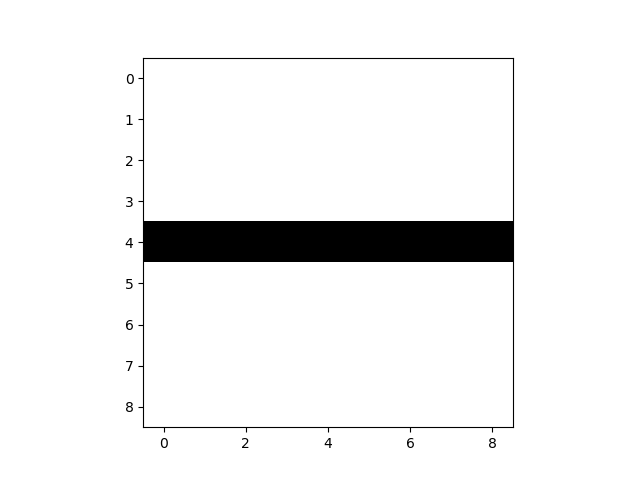
\includegraphics[width=.1\textwidth]{lineAng.input0.pic.png}}
        \subfigure[]{
        \label{fig.picDataAng1}
        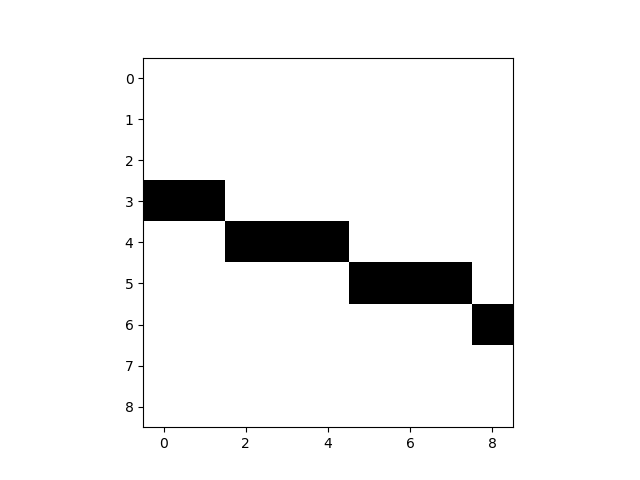
\includegraphics[width=.1\textwidth]{lineAng.input1.pic.png}}
        \subfigure[]{
        \label{fig.picDataAng2}
        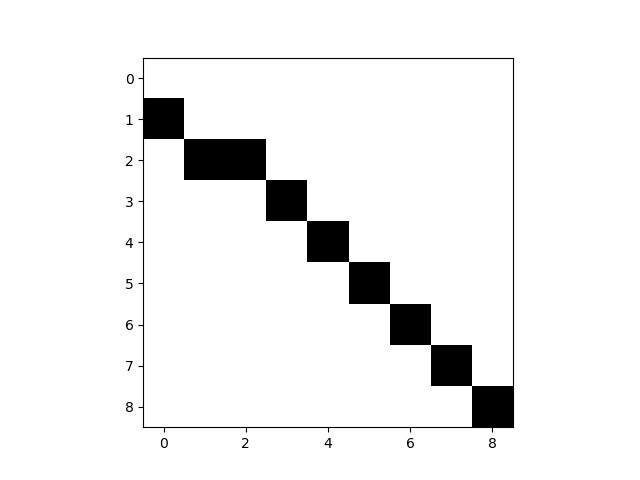
\includegraphics[width=.1\textwidth]{lineAng.input2.pic.png}}
        \subfigure[]{
        \label{fig.picDataAng3}
        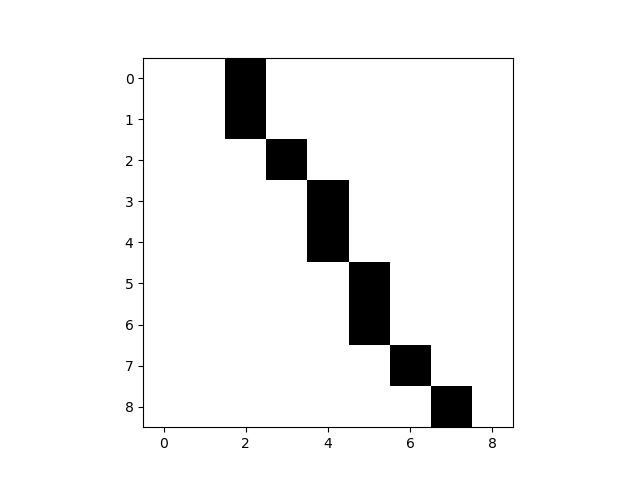
\includegraphics[width=.1\textwidth]{lineAng.input3.pic.png}}
        \subfigure[]{
        \label{fig.picDataAng4}
        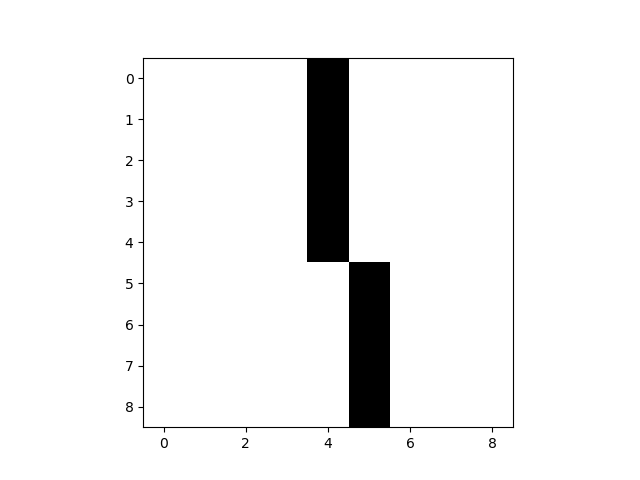
\includegraphics[width=.1\textwidth]{lineAng.input4.pic.png}}
        \subfigure[]{
        \label{fig.picDataAng5}
        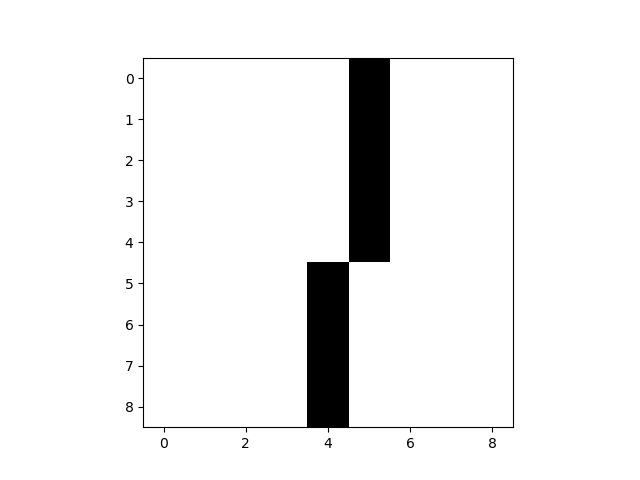
\includegraphics[width=.1\textwidth]{lineAng.input5.pic.png}}
        \subfigure[]{
        \label{fig.picDataAng6}
        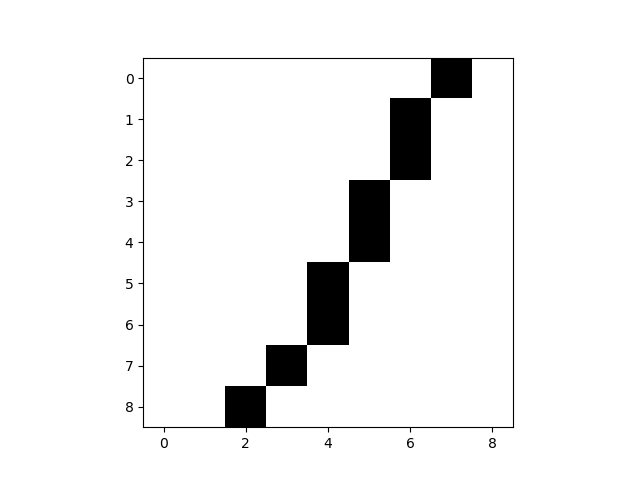
\includegraphics[width=.1\textwidth]{lineAng.input6.pic.png}}
        \subfigure[]{
        \label{fig.picDataAng7}
        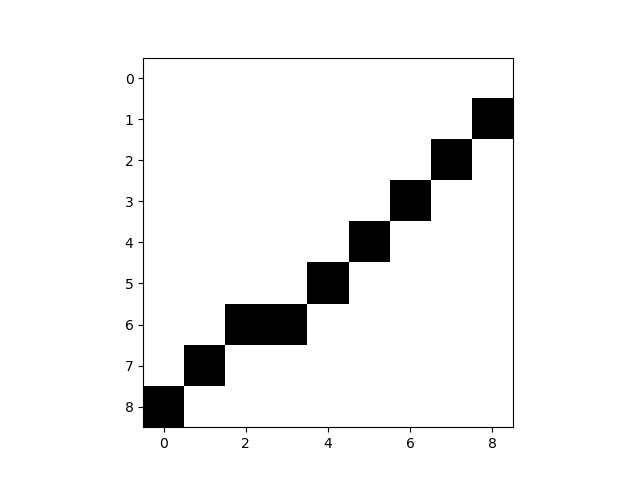
\includegraphics[width=.1\textwidth]{lineAng.input7.pic.png}}
        \subfigure[]{
        \label{fig.picDataAng8}
        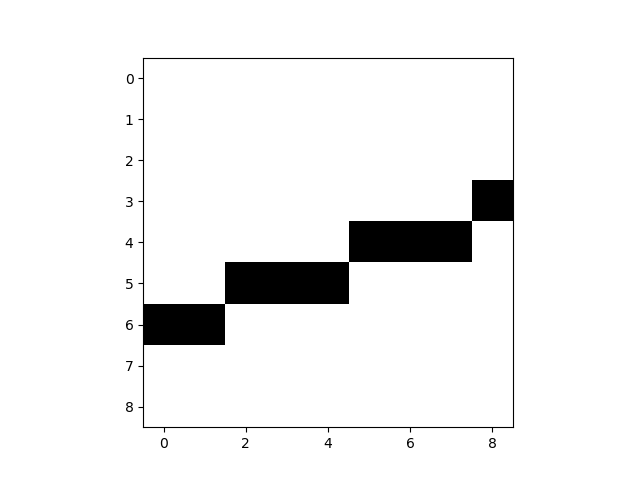
\includegraphics[width=.1\textwidth]{lineAng.input8.pic.png}}
        \subfigure[]{
        \label{fig.picDataPos0}
        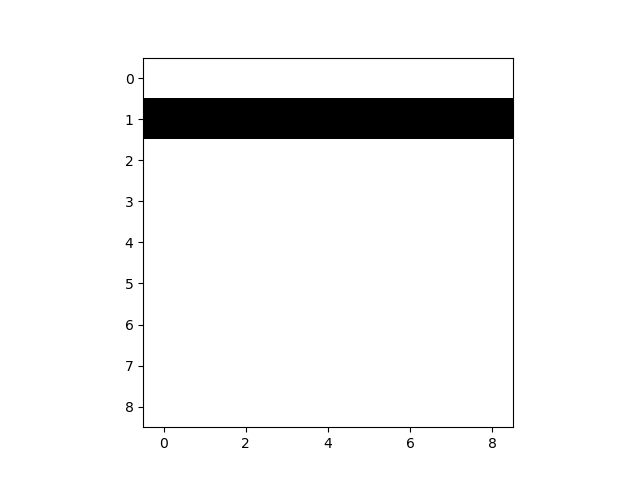
\includegraphics[width=.1\textwidth]{linePos.input0.pic.png}}
        \subfigure[]{
        \label{fig.picDataPos1}
        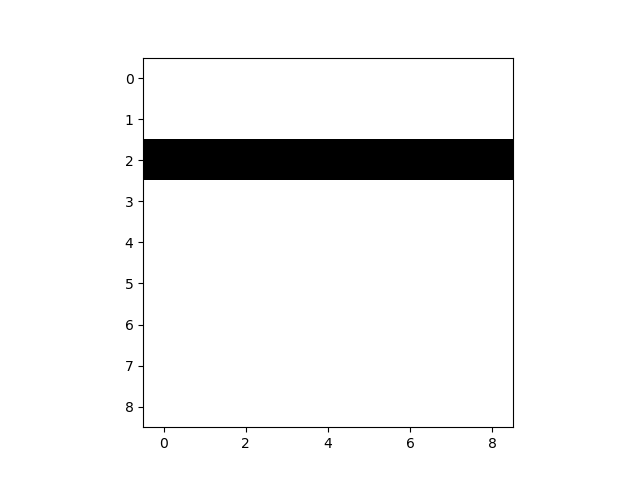
\includegraphics[width=.1\textwidth]{linePos.input1.pic.png}}
        \subfigure[]{
        \label{fig.picDataPos2}
        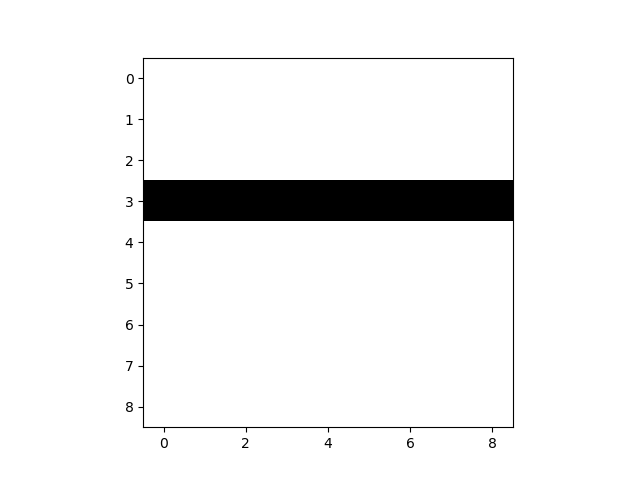
\includegraphics[width=.1\textwidth]{linePos.input2.pic.png}}
        \subfigure[]{
        \label{fig.picDataPos3}
        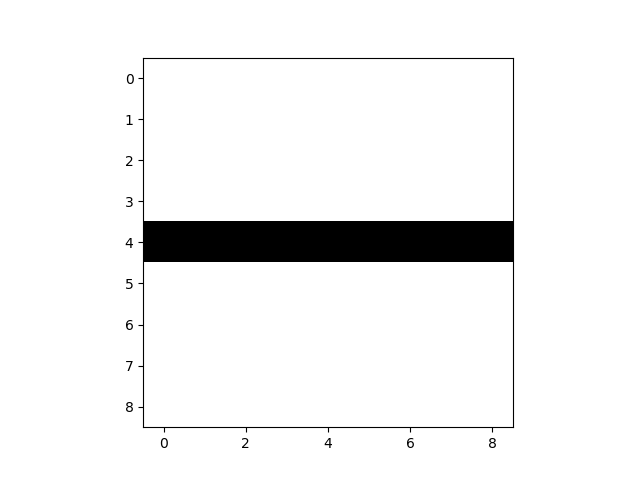
\includegraphics[width=.1\textwidth]{linePos.input3.pic.png}}
        \subfigure[]{
        \label{fig.picDataPos4}
        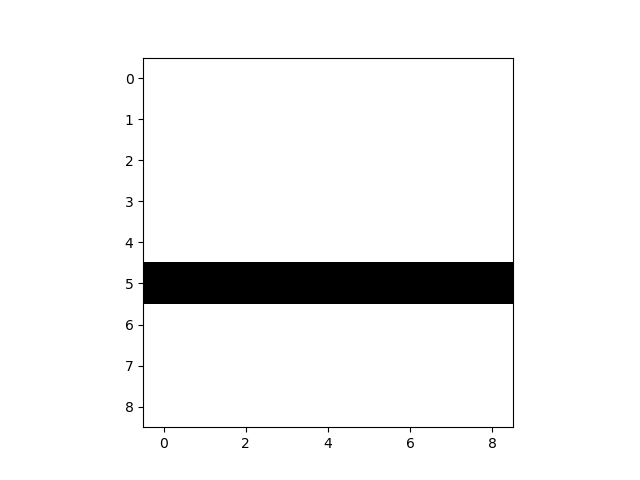
\includegraphics[width=.1\textwidth]{linePos.input4.pic.png}}
        \subfigure[]{
        \label{fig.picDataPos5}
        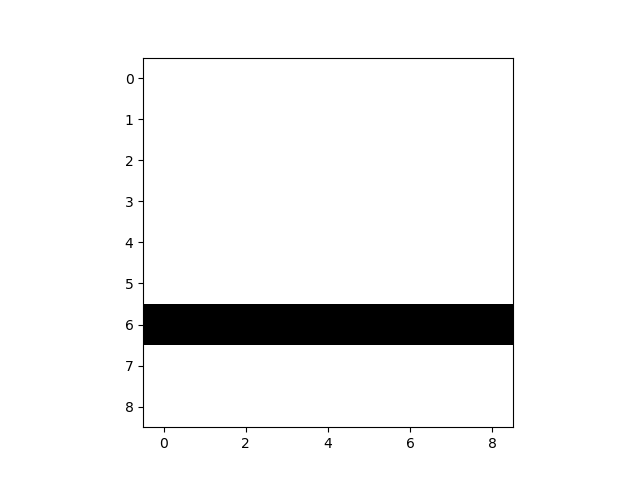
\includegraphics[width=.1\textwidth]{linePos.input5.pic.png}}
        \subfigure[]{
        \label{fig.picDataPos6}
        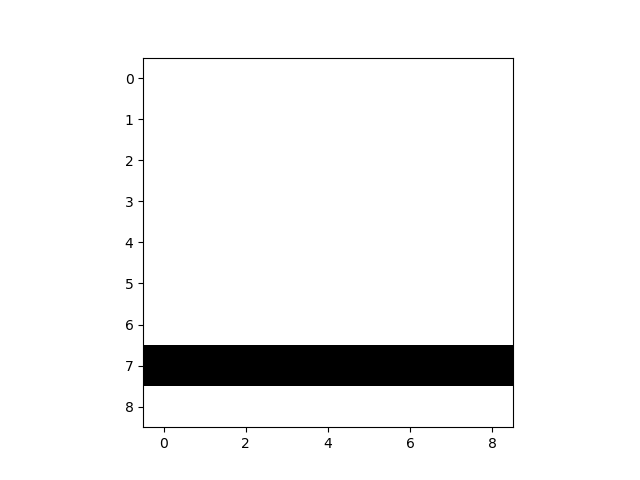
\includegraphics[width=.1\textwidth]{linePos.input6.pic.png}}
        \caption{inputs of line detector networks}
        \label{fig.picData}
    \end{figure}
    
    \begin{figure}[htbp]
    \centering
        \subfigure[spiking rate for different line positions]{
        \label{fig.lineAngRate}
        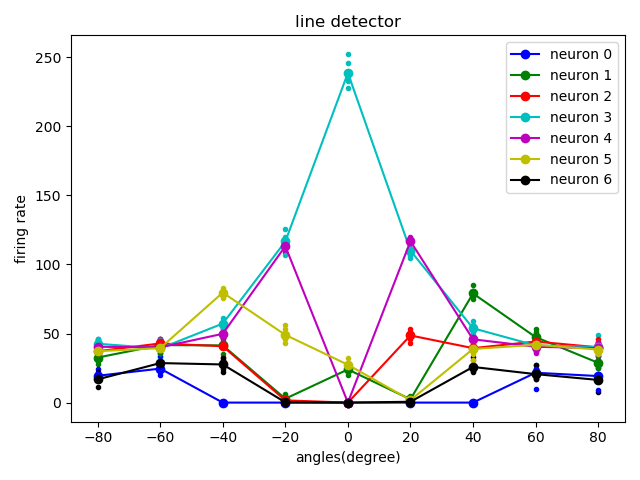
\includegraphics[width=.48\textwidth]{lineAng.iter4.rate.png}}
        \subfigure[spiking rate for different line positions]{
        \label{fig.linePosRate}
        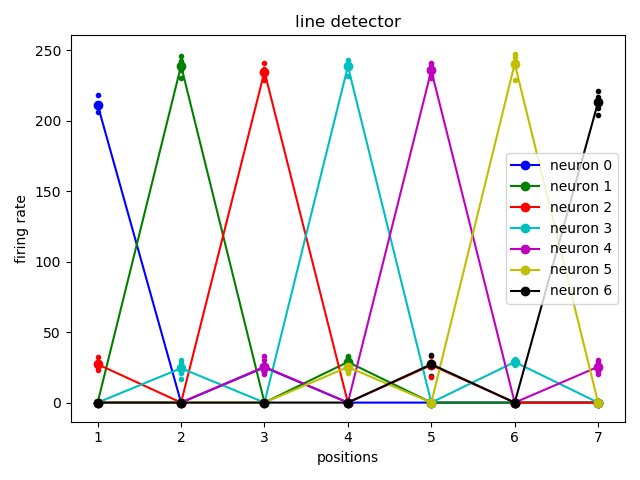
\includegraphics[width=.48\textwidth]{linePos.iter4.rate.png}}
        \caption{averaged spiking rate of line detector neurons of 5 iterations}
        \label{fig.lineRate}
    \end{figure}
    
    Note that neuron $4$ is potentially excited with the input as Fig. \ref{fig.picDataAng1} and Fig. \ref{fig.picDataAng8}, because these two inputs cantains a line segment at row $5$. But the firing rate is still under \texttt{150 Hz}, which does not violate the output decoding threshold.

	\bibliography{ref}
    \bibliographystyle{acl_natbib}
\end{document}